\documentclass[10pt,a4paper]{article}
\usepackage[ansinew]{inputenc} 
\usepackage[T1]{fontenc} 
\usepackage[danish]{babel}				% Dansk ordbog
\usepackage{amsmath, amsfonts, amssymb} % Matematiske pakker
\usepackage{graphicx} 					% Grafiksk pakke
\usepackage{float}						% TIL AT BILLEDER BLIVER HVOR DE ER

\usepackage[left	=3cm,
			right	=2cm,
			top		=2.2cm,
			bottom	=2cm
		]{geometry} 					% Sidejustering

%Mellemrum mellem linjerne
\usepackage{setspace}
\setstretch{1.5} %Afstanden

\usepackage{lastpage}

% Links
\usepackage{hyperref}
\hypersetup{ 
	colorlinks	= true, 	% false: boxed links; true: colored links
    urlcolor	= blue,		% color of external links
    linkcolor	= black, 	% color of page numbers
}

% Figur der st�r vilk�rligt
\usepackage{wrapfig}
%\begin{wrapfigure}{r}{0.6\textwidth}
%	\centering
%	\includegraphics[scale=0.25]{...}
%    \vspace{-20pt}
%    \caption{...}
%  \label{fig:...}
%  \vspace{-10pt}
%\end{wrapfigure}

% Sideops�tning
\usepackage{fancyhdr}					% Header-style
\pagestyle{fancy}
\fancyhf{} % slet alt
\fancyfoot[C]{Side \thepage \text{ af} \pageref{LastPage}} % sidetallet yderst
\lhead[]{\leftmark} % lige side, kapitel titel
\headheight = 35pt
\textheight = 680pt
\footskip 	= 40pt
\rhead{
\begin{picture}(0,0)
\put(-120,0){ 
\includegraphics[scale=0.2]{Diagrammer/Billeder/au-ingenioerhoejskolen_da.jpg}}
\end{picture}}
\renewcommand{\headrulewidth}{0.4pt}
\renewcommand{\footrulewidth}{0.4pt}

\usepackage{enumerate}

\usepackage{subfiles}

%----------------------------------------------------------
% F�lgende er til tabeller
%----------------------------------------------------------
\usepackage{booktabs, cellspace} 		
\addtolength\cellspacetoplimit{10pt}
\addtolength\cellspacebottomlimit{10pt}

%----------------------------------------------------------
% F�lgende er til koder.
% Inds�ttes mellem \begin{lstlisting} og \end{lstlisting}
%----------------------------------------------------------
\usepackage{listings}
\usepackage{color}
\usepackage{textcomp}
\definecolor{listinggray}{gray}{0.9}
\definecolor{lbcolor}{rgb}{0.9,0.9,0.9}
\lstset{
	language		= [Sharp]C,
	keywordstyle	= \bfseries\ttfamily\color[rgb]{0,0,1},
	identifierstyle	= \ttfamily,
	commentstyle	= \color[rgb]{0.133,0.545,0.133},
	stringstyle		= \ttfamily\color[rgb]{0.627,0.126,0.941},
	showstringspaces= false,
	basicstyle		= \small,
	numberstyle		= \footnotesize,
	numbers			= left, % Tal? Udkommenter hvis ikke
	stepnumber		= 1,
	numbersep		= 5pt,
	tabsize			= 2,
	breaklines		= true,
	prebreak 		= \raisebox{0ex}[0ex][0ex]{\ensuremath{\hookleftarrow}},
	breakatwhitespace= false,
	aboveskip		= {1.5\baselineskip},
  	columns			= fixed,
  	upquote			= true,
  	extendedchars	= true,
	lineskip		= 1.5pt,
    xleftmargin		= 17pt,
	framexleftmargin= 17pt,
	framexrightmargin	= 5pt,
	framexbottommargin	= 4pt,
% frame=single,
 	backgroundcolor=\color{lbcolor},
}
\renewcommand*{\lstlistingname}{Kodeudsnit}

\usepackage{caption}
\DeclareCaptionFont{white}{\color{white}}
\DeclareCaptionFormat{listing}{\colorbox[cmyk]{0.43, 0.35, 0.35,0.01}{\parbox{\textwidth}{\hspace{15pt}#1#2#3}}}
\captionsetup[lstlisting]{format=listing,labelfont=white,textfont=white, singlelinecheck=false, margin=0pt, font={bf,footnotesize}}


%----------------------------------------------------------
% F�lgende er tabel over Use Cases - Akt�rer - Forventet 
% 	resultat og checkbox
% Inds�ttes med \begin{testcase} og \end{testcase}
%----------------------------------------------------------
%\usepackage{enumitem,calc}

\newenvironment{testcase}[1]
{
\begin{tabular}{| p{1.2cm} | p{6cm} | p{5.5cm} | l|}\hline
\textbf{TRIN} & \textbf{Aktion / Input} & \textbf{Forventet resultat} & \textbf{CHK} \\
\hline
}
{&\\\hline
\end{tabular}
\\\\}
\newcommand\punkt{&\\\hline} 
\newcommand\Aktion{&}
\newcommand\Forventet{&}

%Grader tegn
\newcommand{\degree}{\ensuremath{^\circ}}

%Bilag kommando
\providecommand{\Bilag}
{ 	\cleardoublepage
	\appendix % Sletter alle kapitelnumre og starter forfra
	\renewcommand{\appendixname}{Bilag} % Fort�ller navnet skal v�re "Bilag"
	\part*{Bilag}
	\addcontentsline{toc}{part}{Bilag}
	\renewcommand{\thesection}{\Roman{section}}
}

% Paragraph instillinger
\renewcommand\paragraph{\@startsection{paragraph}{4}{\z@}%
  {-3.25ex\@plus -1ex \@minus -.2ex}%
  {1.5ex \@plus .2ex}%
  {\normalfont\normalsize\bfseries}}
\author{Silver Bullet Sort\\\\Gruppe 5}
\title{Hardware specifikation}
\date{}
\begin{document}
\maketitle

\newpage
\tableofcontents
\newpage

\section{Form�l}
At fastl�gge systemets hardware gr�nseflader
\section{Referencer}
I dette dokument vil der optr�de referencer til f�lgende dokumenter:
\begin{itemize}
\item SBS\_Systemarkitekur
\item V�gtcelle\_doc - DS-MP40
\item Controller-USB, Users Manual -- 100341\_D\_Controller\_USB(0305)
\end{itemize}

\newpage
\section{Oversigt}
Systemet best�r af f�lgende hardwarekomponenter:
\begin{itemize}
\item PC
\item STK500-kit
\item Operationsforst�rker
\item V�gt
\item USB-Controller
\item Transportb�nd
\item Robot
\item Klossensor
\end{itemize}

\begin{figure}[h]
\centering
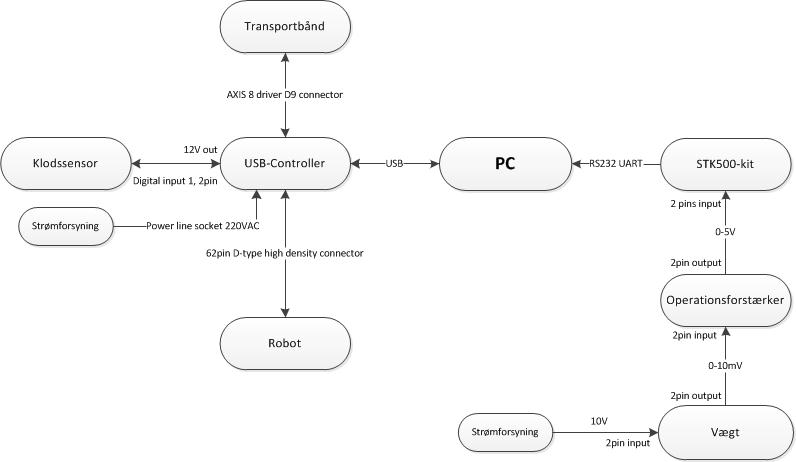
\includegraphics[scale=0.8]{HW_GF.jpg}
\caption{Oversigt over gr�nseflader}
\end{figure}

\section{Hardwarekomponenter}
\subsection{PC}
PC'en er forbundet til USB-Controlleren via et standard USB-stik. USB-controlleren styres med USBC.dll (L�s mere om USBC.dll i \textit{SBS\_Systemarkitektur}.
STK500-kittet er ogs� forbundet til PC'en. Kommunikation sker gennem en RS-232 UART kabel.

\newpage
\subsection{USB-Controller}
Der er en del ind og udgange p� USB-Controlleren. Herunder gives et overblik over USB-Controlleren, f�r de forskellige enheder beskrives kort. Billederne er taget fra USB-Controller manualen. Se n�rmere i dokumentet \textit{Controller-USB, Users Manual -- 100341\_D\_Controller\_USB(0305)}.

\begin{figure}[h]
\centering
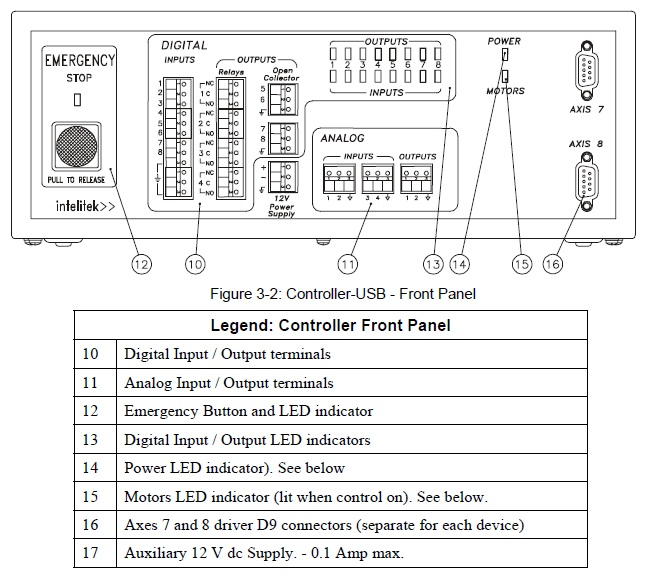
\includegraphics[scale=0.55]{USB-Controller-for.jpg}
\caption{USB-Controller front}
\end{figure}

\begin{figure}[h]
\centering
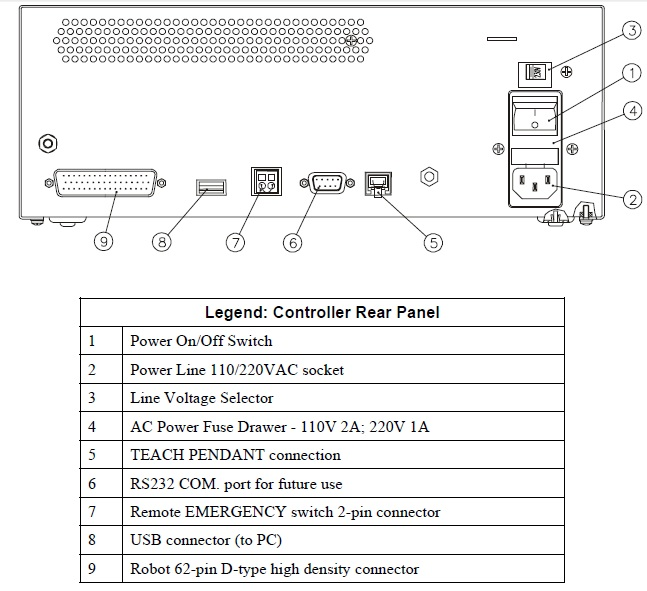
\includegraphics[scale=0.55]{USB-Controller-bag.jpg}
\caption{USB-Controller bagside}
\end{figure}

\subsubsection{Robot}
USB-controlleren er forbundet til robotarmen med en 62-pins type D high density connector.
\subsubsection{Klodssensor}
Klodssensoren g�r ind p� USB-Controllerens Digital input, pin 1 og 2. Derudover benytter sensoren USB-Controllerens 12V output som str�mforsyning.
\subsubsection{Transportb�nd}
Transportb�ndet benytter AXIS 8 driver D9 connectoren p� USB-Controlleren. Transportb�ndet styres ogs� med USBC.dll (L�s mere om USBC.dll i \textit{SBS\_Systemarkitektur}).

\subsection{STK500-kit}
STK500-kittet er forbundet til PC'en via et RS-232 kabel. Der kommunikeres gennem dette via UART'en. 

\subsubsection{V�gt + Operationsforst�rker}
V�gten bruger en str�mkilde p� maksimum 15V, men 10V er dog anbefalet og b�r benyttes.
Outputsp�ndingen er 1mV pr. volt forsyningssp�nding pr kilo. Dvs. at ved et kilo f�r vi en outputsp�nding p� 10mV (for n�rmere information, se databladet \textit{V�gtcelle\_doc - DS-MP40}. STK500-kittet input skal dog v�re i mellem 0-5V, og derfor skal vi forst�rke outputtet fra v�gten, hvilket der bruges en operationsforst�rker til.  

\begin{figure}[h]
\centering
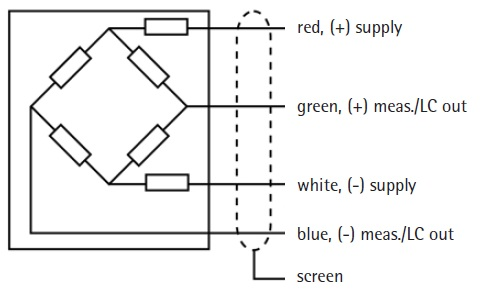
\includegraphics[scale=0.7]{vEgt.jpg}
\caption{V�gt input/output}
\end{figure}

\end{document}